\documentclass[12pt, a3paper]{article}

\usepackage{longtable}
\usepackage{geometry}
	\geometry{top=10mm}
	\geometry{bottom=10mm}
	\geometry{left=5mm}
	\geometry{right=5mm}

\usepackage{graphicx}
\graphicspath{{./images/}}

\newcommand{\scale}{1}

\begin{document}
\pagestyle{empty}

\begin{center}
	\begin{longtable}{c|c||c|c}
	\Large{LEFT} & \Large{RIGHT} & \Large{LEFT} & \Large{RIGHT}\vspace{1ex}\\
	\hline
	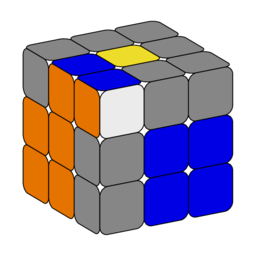
\includegraphics[scale=\scale]{1_left} & 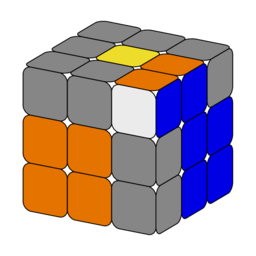
\includegraphics[scale=\scale]{1_right}  &  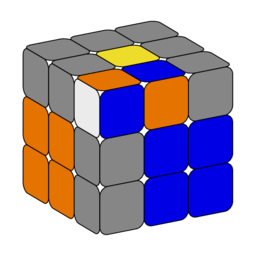
\includegraphics[scale=\scale]{2_left} & 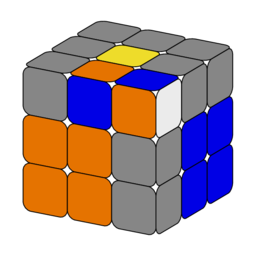
\includegraphics[scale=\scale]{2_right} \\
	U' (L' U L) & U (R U' R') & (L' U L) U' ( ) U2 ( ) & (R U' R') U ( ) U2 ( ) \\
	\hline
	\hline
	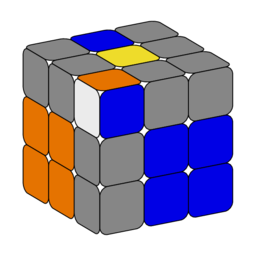
\includegraphics[scale=\scale]{3_left} & 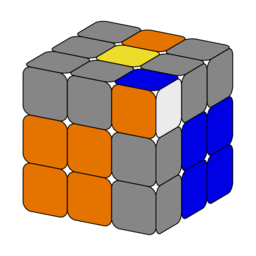
\includegraphics[scale=\scale]{3_right}  &  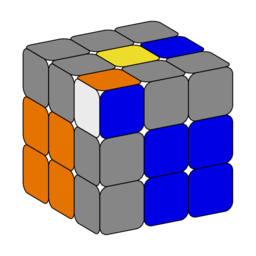
\includegraphics[scale=\scale]{4_left} & 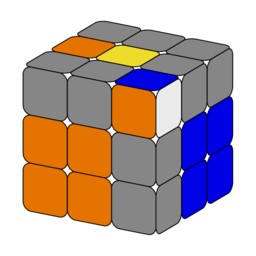
\includegraphics[scale=\scale]{4_right} \\
	(L' U' L) & (R U R') & U (L' U' L) U' ( ) & U' (R U R') U ( ) \\
	\hline
	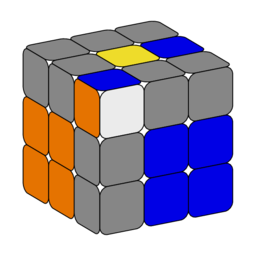
\includegraphics[scale=\scale]{5_left} & 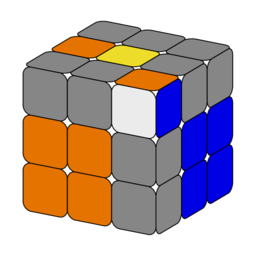
\includegraphics[scale=\scale]{5_right}  &  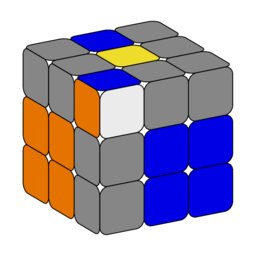
\includegraphics[scale=\scale]{6_left} & 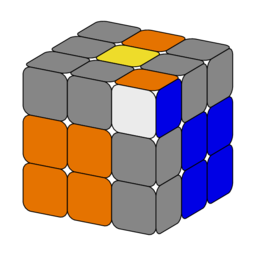
\includegraphics[scale=\scale]{6_right} \\
	U (L' U2 L) U2 (U) & U' (R U2 R') U2 (U') & U (L' U' L) U2 (U) & U' (R U R') U2 (U') \\
	\hline
	\hline
	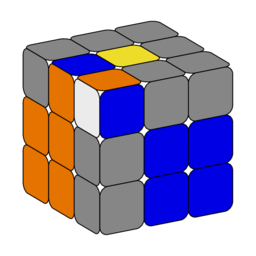
\includegraphics[scale=\scale]{7_left} & 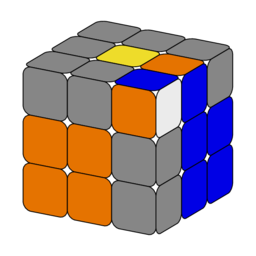
\includegraphics[scale=\scale]{7_right}  &  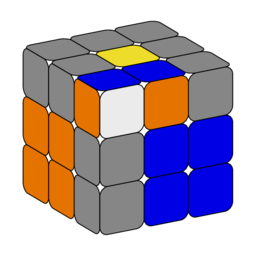
\includegraphics[scale=\scale]{8_left} & 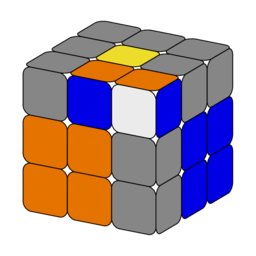
\includegraphics[scale=\scale]{8_right} \\
	U (L' U L) U' (U') & U' (R U' R') U (U) & (L' U' L) U2 (U) U' (U) & (R U R') U2 (U') U (U') \\
	\hline
	\hline
	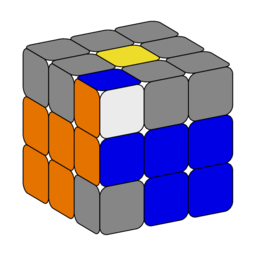
\includegraphics[scale=\scale]{9_left} & 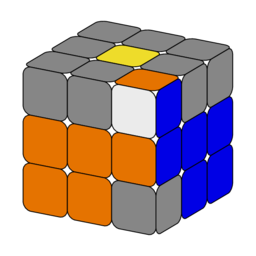
\includegraphics[scale=\scale]{9_right}  &  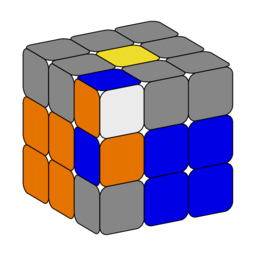
\includegraphics[scale=\scale]{10_left} & 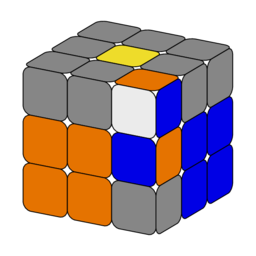
\includegraphics[scale=\scale]{10_right} \\
	U (L' U L) U2 ( ) & U' (R U' R') U2 ( ) & U (L' U' L) y' U' [R U R'] & U' (R U R') y U [L' U' L] \\
	\hline
	\hline
	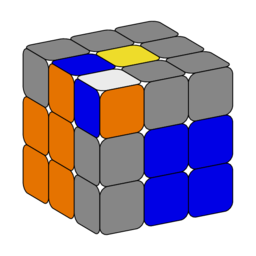
\includegraphics[scale=\scale]{11_left} & 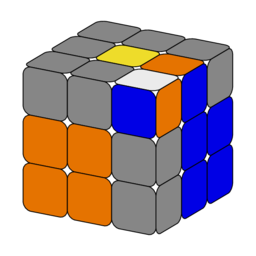
\includegraphics[scale=\scale]{11_right}  &  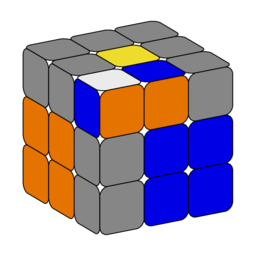
\includegraphics[scale=\scale]{12_left} & 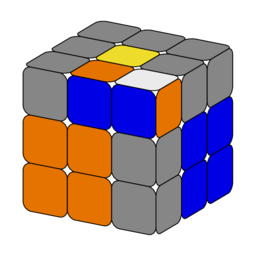
\includegraphics[scale=\scale]{12_right} \\
	(L' U2 L) U (U') & (R U2 R') U' (U) & (L' U' L) U2 ( ) U ( ) & (R U R') U2 ( ) U' ( ) \\
	\hline
	\hline
	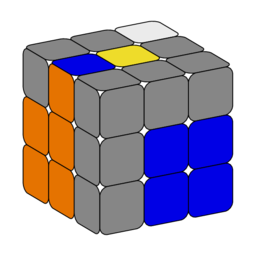
\includegraphics[scale=\scale]{13_left} & 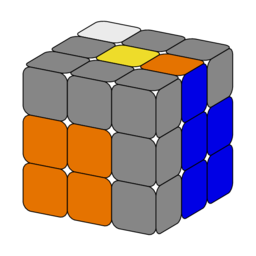
\includegraphics[scale=\scale]{13_right}  &  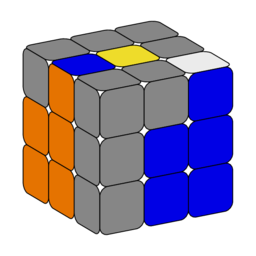
\includegraphics[scale=\scale]{14_left} & 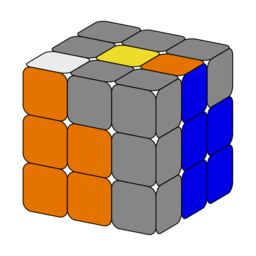
\includegraphics[scale=\scale]{14_right} \\
	(L' U' L) U' (U) & (R U R') U (U') & (L' U2 L) U' (U) & (R U2 R') U (U') \\
	\hline
	\hline
	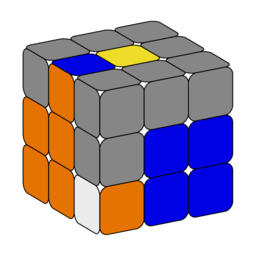
\includegraphics[scale=\scale]{15_left} & 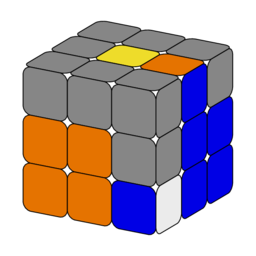
\includegraphics[scale=\scale]{15_right}  &  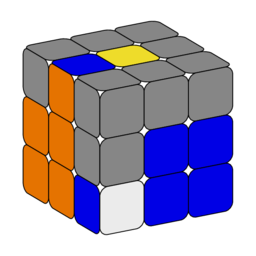
\includegraphics[scale=\scale]{16_left} & 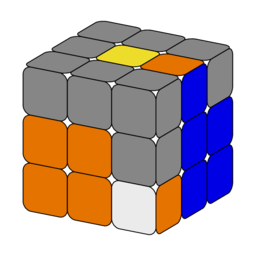
\includegraphics[scale=\scale]{16_right} \\
	(L' U' L) U ( ) & (R U R') U' ( ) & (L' U L) U' ( ) & (R U' R') U ( ) \\
	\hline
	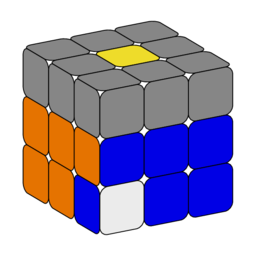
\includegraphics[scale=\scale]{17_left} & 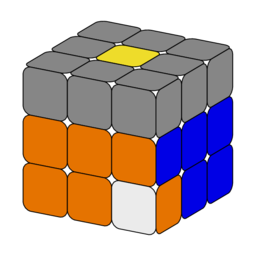
\includegraphics[scale=\scale]{17_right}  &  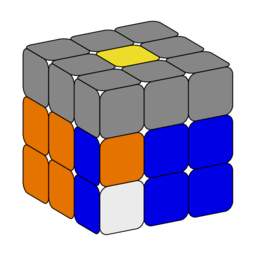
\includegraphics[scale=\scale]{18_left} & 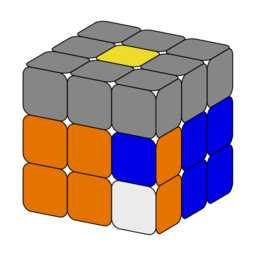
\includegraphics[scale=\scale]{18_right} \\
	(L' U L) U (U') U2 ( ) & (R U' R') U' (U) U2 ( ) & (L' U L) U ( ) y' U' [R U R'] & (R U' R') U' ( ) y U [L' U' L] \\
	\hline
	\hline
	& & 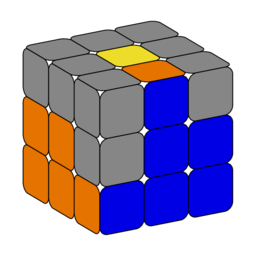
\includegraphics[scale=\scale]{19_left} & 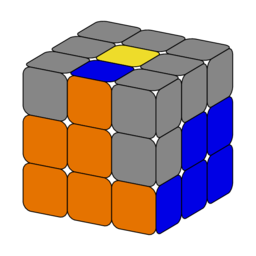
\includegraphics[scale=\scale]{19_right} \\
	& & U' (L' U L) U y' [R U' R'] & U (R U' R') U' y [L' U L] \\
	\hline
	\end{longtable}
	% Non-symetrical positions
	\begin{tabular}{c|c|c}
		\hline
		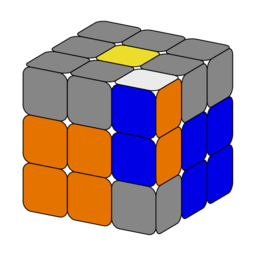
\includegraphics[scale=\scale]{20_right} & 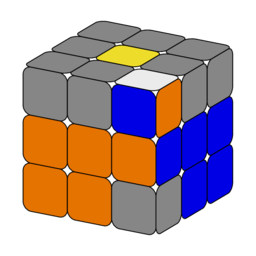
\includegraphics[scale=\scale]{21_right} & 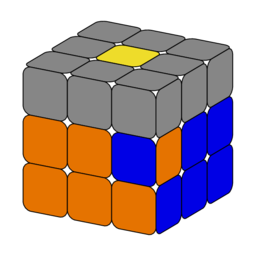
\includegraphics[scale=\scale]{22_right} \\
		(R U R') U' ( ) U' ( ) & U (R U2 R') y [L' U' L] & (R U' R') U y' [R' U2 R] U2 [U] \\
		\hline
	\end{tabular}
\end{center}
\end{document}
